\section{Implementation Details}

\subsection{VLM prompting}
\TODO{REPLACE}

\noindent\fbox{\parbox{0.97\linewidth}{\scriptsize{\texttt{{% <-- removes unnecessary first line indent
- Vision input: <RGB image observation> \\
- Text input: It is a <target object>. There is <GAPart Segmentation> on it. Please provide a detailed and accurate description of the scene which may help me with operating this object.
}}}}}

For example, the input image is Fig.~\ref{fig:example_VLM} and the prompt and output are:

\begin{figure}[h]
    \centering
    \vspace{-4ex}
    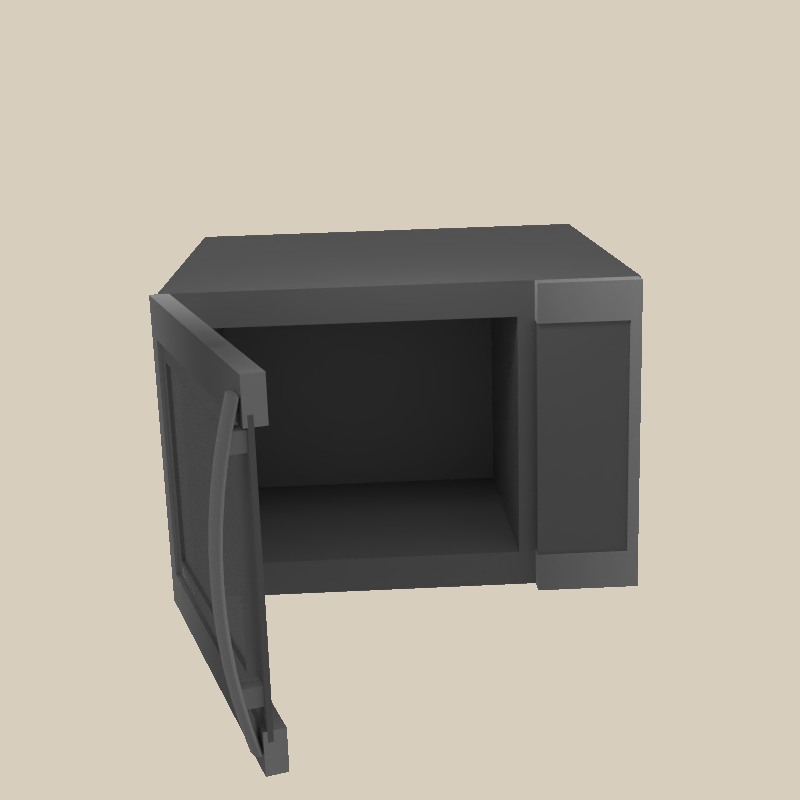
\includegraphics[width=0.5\linewidth]{Microwave_7310_00_027_raw.png}
    \caption{Example RGB image input for VLM}
    \label{fig:example_VLM}
    \vspace{-4ex}
\end{figure}

\noindent\fbox{\parbox{0.97\linewidth}{\scriptsize{\texttt{{% <-- removes unnecessary first line indent
- Text input: It is a microwave. There is a door and a handle on it. Please provide a detailed and accurate description of the scene which may help me with operating this object. \\
- Output: It is a microwave with a door and handle on it. The microwave is made of silver metal and has a smooth surface. The door is open, revealing the interior of the microwave. The handle is on the door, allowing someone to open and close the door. The microwave is on a beige background.
}}}}}

\subsection{LLM prompting}

\todo{
\begin{itemize}
    \item Output Format Description: This part provides the LLM with the standard output format.
    \item Examples: A diverse range of input-output pairs are provided to help the LLM understand. These include tasks that involve manipulating various objects and parts, tasks with scene descriptions, tasks with a manual, and tasks that require a single step, multiple steps, and multiple strategies.
    \item Failure Cases: We additionally present some incorrect outputs for the LLM. Analyzing these cases aids in improving the quality of the LLM's output.
\end{itemize}
}


\noindent\fbox{\parbox{0.97\linewidth}{\scriptsize{\texttt{{% <-- removes unnecessary first line indent
As an advanced and capable artificial entity, you are tasked with generating instructions to interact with a multitude of articulated objects. These encompass a wide range of items such as Box, Bucket, Camera, Coffee Machine, Dishwasher, Door, Keyboard, Kitchen Pot, Laptop, Microwave, Oven, Phone, Printer, Refrigerator, Remote, Safe, Storage Furniture, Suitcase, Table, Toaster, Toilet, Trash Can, Washing Machine, and others. \\
\\
Your duty is to generate all conceivable actions pertaining to the components of these objects, such as a door, in order to accomplish the tasks assigned to you. Additionally, you are obliged to articulate the direction of the interaction. The term "+" is employed to signify the action of distancing the part from the object, whereas "-" implies drawing the part closer to the object's main body.\\
\\
You may also be provided with a description of the scene to facilitate your planning. This is optional, but if it is provided, it will facilitate your decision.\\
\\
To elucidate, consider the following examples:\\
\\
Instruction: Open the cabinet. Description: There are 3 drawers, 3 handles in the scene.\\
\\
Output:
Strategy 1: 1 step: (1) (Drawer, prismatic, +)\\
\\
Strategy 2: 1 step: (1) (Handle, prismatic, +)\\
\\
Instruction: Open the cabinet. Description: There are 2 doors, 2 handles in the scene.\\
\\
Output:
Strategy 1: 1 step: (1) (Door, revolute, +)\\
\\
Strategy 2: 1 step: (1) (Handle, revolute, +)\\
\\
Instruction: Close the door. Description: There are 1 door, 1 handle in the scene.\\
\\
Output:
Strategy 1: 1 step: (1) (Door, revolute, -)\\
\\
Instruction: Open the microwave. Description: There are 1 door, 10 buttons in the scene.\\
\\
Output:
Strategy 1: 1 step: (1) (Door, revolute, +)
Strategy 2: 2 steps: (1) (Button, prismatic, -) (2) (Door, revolute, +)
Strategy 3: 1 step: (1) (Button, prismatic, -)\\
\\
More instructions will be subsequently provided to you. It is expected of you to adhere to the outlined output format and generate as many potential answers as feasible. Please note that each action is constituted by a part, a joint type(prismatic or revolute) and a direction, so the following answers is not encouraged:\\
\\
Instruction: Open the microwave .Description: There is 1 door, and 10 buttons in the scene.\\
\\
Output:
Strategy 1: 1 step: (1) (Microwave, revolute, +)
This is not good because microwave is not a part in microwave. A part is a part of an object, for example, door, drawer, button, lid, handle, hinge, knob.\\
\\
Furthermore, as you are aware, there is the potential for specific steps to fail during the robot's task completion. Should such a failure occur, I will provide a comprehensive account of the issue, thereby enabling you to devise a more effective solution informed by this new knowledge of the failure. \\
% }}}}}
% \noindent\fbox{\parbox{0.97\linewidth}{\scriptsize{\texttt{{% <-- removes unnecessary first line indent
For example, when you are opening a microwave with the following steps:\\
\\
Strategy: 1 step: (1) (Door, revolute, +)\\
\\
then I tell you:
Failure: It fails when opening the door
you can answer:
New Strategy 1: 2 steps: (1) (Button, prismatic, -) (2) (Door, revolute,  +)
New Strategy 2: 1 step: (1) (Button, prismatic, -)
}}}}}\\